%File: anonymous-submission-latex-2023.tex
\documentclass[letterpaper]{article} % DO NOT CHANGE THIS
\usepackage[]{aaai23}  % DO NOT CHANGE THIS
\usepackage{times}  % DO NOT CHANGE THIS
\usepackage{helvet}  % DO NOT CHANGE THIS
\usepackage{courier}  % DO NOT CHANGE THIS
\usepackage[hyphens]{url}  % DO NOT CHANGE THIS
\usepackage{graphicx} % DO NOT CHANGE THIS
\urlstyle{rm} % DO NOT CHANGE THIS
\def\UrlFont{\rm}  % DO NOT CHANGE THIS
\usepackage{natbib}  % DO NOT CHANGE THIS AND DO NOT ADD ANY OPTIONS TO IT
\usepackage{caption} % DO NOT CHANGE THIS AND DO NOT ADD ANY OPTIONS TO IT
\frenchspacing  % DO NOT CHANGE THIS
\setlength{\pdfpagewidth}{8.5in} % DO NOT CHANGE THIS
\setlength{\pdfpageheight}{11in} % DO NOT CHANGE THIS
%
% These are recommended to typeset algorithms but not required. See the subsubsection on algorithms. Remove them if you don't have algorithms in your paper.
\usepackage{algorithm}
\usepackage{algorithmic}
\usepackage{amsmath}
\usepackage{hyperref} 
% \usepackage[backref]{hyperref} 
\usepackage{stfloats}
\usepackage{booktabs}
\usepackage{subfigure}
\usepackage{cleveref}
\usepackage{xcolor}
\usepackage{multirow}

% \usepackage{multicolumn}
% \usepackage{subcaption}
% \usepackage{float}
%
% These are are recommended to typeset listings but not required. See the subsubsection on listing. Remove this block if you don't have listings in your paper.
\usepackage{newfloat}
\usepackage{appendix}
\usepackage{listings}
\DeclareCaptionStyle{ruled}{labelfont=normalfont,labelsep=colon,strut=off} % DO NOT CHANGE THIS
\lstset{%
    basicstyle={\footnotesize\ttfamily},% footnotesize acceptable for monospace
    numbers=left,numberstyle=\footnotesize,xleftmargin=2em,% show line numbers, remove this entire line if you don't want the numbers.
    aboveskip=0pt,belowskip=0pt,%
    showstringspaces=false,tabsize=2,breaklines=true}
\floatstyle{ruled}
\newfloat{listing}{tb}{lst}{}
\floatname{listing}{Listing}

\newcommand{\hide}[1]{}
\newcommand{\red}[1]{{\leavevmode\color{red}{#1}}}
\newcommand{\hui}[1]{\textcolor{red}{[Hui: #1]}}
\newcommand{\revised}[1]{\textcolor{blue}{#1}}


\newcommand{\myauthornote}[3]{{\color{#2} {\sc #1}: #3}}
\newcommand{\authorText}[2]{{\color{#1}#2}}
\newcommand\yl[1]{\myauthornote{yl}{orange}{#1}}

%
% Keep the \pdfinfo as shown here. There's no need
% for you to add the /Title and /Author tags.
\pdfinfo{
/TemplateVersion (2023.1)
}

% DISALLOWED PACKAGES
% \usepackage{authblk} -- This package is specifically forbidden
% \usepackage{balance} -- This package is specifically forbidden
% \usepackage{color (if used in text)
% \usepackage{CJK} -- This package is specifically forbidden
% \usepackage{float} -- This package is specifically forbidden
% \usepackage{flushend} -- This package is specifically forbidden
% \usepackage{fontenc} -- This package is specifically forbidden
% \usepackage{fullpage} -- This package is specifically forbidden
% \usepackage{geometry} -- This package is specifically forbidden
% \usepackage{grffile} -- This package is specifically forbidden
% \usepackage{hyperref} -- This package is specifically forbidden
% \usepackage{navigator} -- This package is specifically forbidden
% (or any other package that embeds links such as navigator or hyperref)
% \indentfirst} -- This package is specifically forbidden
% \layout} -- This package is specifically forbidden
% \multicol} -- This package is specifically forbidden
% \nameref} -- This package is specifically forbidden
% \usepackage{savetrees} -- This package is specifically forbidden
% \usepackage{setspace} -- This package is specifically forbidden
% \usepackage{stfloats} -- This package is specifically forbidden
% \usepackage{tabu} -- This package is specifically forbidden
% \usepackage{titlesec} -- This package is specifically forbidden
% \usepackage{tocbibind} -- This package is specifically forbidden
% \usepackage{ulem} -- This package is specifically forbidden
% \usepackage{wrapfig} -- This package is specifically forbidden
% DISALLOWED COMMANDS
% \nocopyright -- Your paper will not be published if you use this command
% \addtolength -- This command may not be used
% \balance -- This command may not be used
% \baselinestretch -- Your paper will not be published if you use this command
% \clearpage -- No page breaks of any kind may be used for the final version of your paper
% \columnsep -- This command may not be used
% \newpage -- No page breaks of any kind may be used for the final version of your paper
% \pagebreak -- No page breaks of any kind may be used for the final version of your paperr
% \pagestyle -- This command may not be used
% \tiny -- This is not an acceptable font size.
% \vspace{- -- No negative value may be used in proximity of a caption, figure, table, section, subsection, subsubsection, or reference
% \vskip{- -- No negative value may be used to alter spacing above or below a caption, figure, table, section, subsection, subsubsection, or reference

\setcounter{secnumdepth}{2} %May be changed to 1 or 2 if section numbers are desired.

% The file aaai23.sty is the style file for AAAI Press
% proceedings, working notes, and technical reports.
%

% Title

% Your title must be in mixed case, not sentence case.
% That means all verbs (including short verbs like be, is, using,and go),
% nouns, adverbs, adjectives should be capitalized, including both words in hyphenated terms, while
% articles, conjunctions, and prepositions are lower case unless they
% directly follow a colon or long dash
\title{Accuracy Improvement of Code Search Based on Generative Adversarial Network }


\author{Sheng Zhang 23020221154146\\Min-Hua Zheng 23020221154151\\Yu-Bin Zhang 23020221154149}




% \email{sheng@stu.xmu.edu.cn}
% \authornotemark[1]
% \affiliation{%
%     \institution{Xiamen university}
%     \country{China}
% }


\begin{document}

\maketitle
    %!TEX root = ../main_article.tex

\begin{abstract}
    Code search is a foundational task in software development, which studies semantic similarity between natural language queries and program code. Recent years have witnessed great progress made in code search. However, researchers tend to pre-train a code representation model in different program languages so that it can be used in code related downstream problems and then fine-tune it in code search with a specific program language. Our empirical study shows that there may be performance damage when fine-tuning code search in multiple program languages. We believe that it is caused by the entanglement between code identity information and code semantic information. Therefore, we proposed a search enhancement framework based on GAN, so as to reduce identity information provided by pretrained models. Our framework contains two networks: one is a generator, of which the intention is to generate code embedding vectors without identity information, and the other is a discriminator, aiming at recognizing whether there is identity information.
\end{abstract}
    %!TEX root = ../main_article.tex

\section{Introduction}
\label{section:1}

Code search plays a vital role in the software development process, which is an essential field of Software Engineering and studies the semantic similarity between natural language queries and program code. Recent years have witnessed a massive increment in source code. The statistic shows that more than 60 million new projects were created only in 2020 (\citealp{abs-2110-10246}). Thus, code search engines can improve the development efficiency of program developers, enabling them to search for existing code or examples of some API (Application Programming Interface) instead of “rebuilding wheels.” 

As deep learning has grown by leaps and bounds in recent years, a number of methods have been proposed in code search, such as Recurrent Neural Network (RNN) based models (\citealp{DeepCS}), CNNs (Convolutional Neural Networks) based models (\citealp{CQIL, ShuaiX0Y0L20}), graph based models (\citealp{, GuCM21}), and Pre-trained Language Models (PLMs) based models (\citealp{CodeBERT,CoCLR,GraphCodeBERT,UniXcoder}). 

From the view of PLMs, all of them have well performance in code search, with complex model architecture and advanced training techniques. However, PLMs often treat code search as a downstream task, which means researchers can pre-train a model with hybrid objectives and multiple program language code data, then fine-tune it in a specific program language for code search (\citealp{UniXcoder,CodeBERT,GraphCodeBERT,SPTCode}). Our empirical study shows that there might be a performance decline when fine-tuning with data in multiple languages. Table~\ref{tab:comparison} shows MRR (Mean Reciprocal Rank, \citealp{MRR}) comparisons between single program language fine-tuned models, and multiple program language fine-tuned models. The left first column indicates what program languages have been used in fine-tuning and the rest columns show the search performance toward a specific language according to the first column. Similar to multilingual models (\citealp{multilingualModel,YangYCD21}), code information can be roughly divided into identity information, distinguishing code from another code written in different program languages, and semantic information, which reveals its intention and with a corresponding natural language description. In code search, code semantic information is only needed, for it is matched with specific queries. The identity information may confound model training and decrease performance when fine-tuning with multiple program language data. We view identity information as the signal that helps to distinguish different program language data, which has the same idea as classification. Semantic information reveals the code intention, which is related to code search.
% \begin{figure}[htb]
% 	\centering
% 	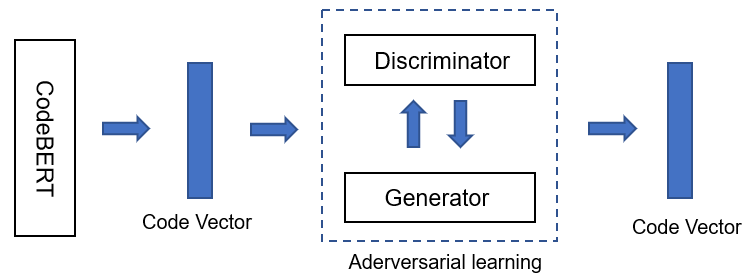
\includegraphics[width=1\linewidth]{imgs/structure.png}
% 	% \vspace{-15pt}
% 	\caption{Structure of the search enhancement framework.}
% 	% \vspace{-12pt}
% 	\label{fig:structure}
% \end{figure}

Therefore, we want to reduce the identity information of the embedding vector given by code search pre-trained models. We propose two strategies for disentangling.  The first is to follow the idea of GAN (Generative Adversarial Network, \citealp{goodfellow2020generative}) and leverage a generator to generate identity free embedding vectors. The second is to use an additional network to obtain identity and semantic vectors separately. We consider maximizing KL divergence in the loss function.

In summary, our contributions are:
\begin{enumerate} 
\item Reveal the performance decline problem that appears when fine-tuning code search with multiple program languages.
\item We propose different disentangling strategies for splitting identity and semantic information of the embedding vectors output by pre-train code models.
\end{enumerate}


% Table generated by Excel2LaTeX from sheet 'Sheet1'
\begin{table}[htbp]
	\centering
	\caption{Performance comparisons with different fine-tuning program languages}
	\vspace{-5pt}
	\resizebox{\linewidth}{!}{
	\begin{tabular}{lrrrr}
		\toprule
        & Python & Go  & Java & PHP \\
    \midrule
    Python & 0.369 & \_  & \_  &  \\
    Go  & \_  & 0.904 & \_  & \_ \\
    Java & \_  & \_  & 0.764 & \_ \\
    PHP & \_  & \_  & \_  & 0.708 \\
    Python\_Java & 0.468 & \_  & 0.708 $\downarrow$ & \_ \\
    Python\_Go & 0.404 & 0.882 $\downarrow$ & \_  & \_ \\
    Java\_Go & \_  & 0.902 $\downarrow$ & 0.724 $\downarrow$ & \_ \\
    Java\_PHP & \_  & \_  & 0.743 $\downarrow$ & 0.707 $\downarrow$ \\
    Java\_Python\_Go & 0.571 & 0.889 $\downarrow$ & 0.701 $\downarrow$ & \_ \\
    \bottomrule
	\end{tabular}%
	}
	\label{tab:comparison}%
	\vspace{-10	pt}
\end{table}%

    %!TEX root = ../main_article.tex

\section{Related Work}

% In this section, we introduce existing code search methods and machine learning debiasing methods. 
% code search methods

Our work is closely related to the following two domains:

\vspace{3pt}
\noindent\textbf{Code Search.} There is a tremendous amount of research on code search. 
Early works adopt traditional information retrieval methods like Boolean Model~\cite{SaltonFW83}, Vector Space Model~\cite{SaltonWY75} 
and Structural Semantic Indexing~\citep{Dumais04} to estimate 
the relevance between the query and a code snippet~\citep{LvZLWZZ15,BajracharyaOL10}.
Recent works adopt deep neural networks to embed query and code into vectors.
Then, the code search task is performed by measuring the similarity 
(e.g., cosine similarity) between vectors.
% \yl{some are bi-encoder architecture, as described here, but many are cross-encoder architecture such as CodeBERT. Should describe them separately.}
Along this direction, various deep learning based code search methods have been proposed, 
including but not limited to 
recurrent neural network (RNN) based approaches~\citep{DeepCS}, 
convolutional neural network (CNN) based approaches~\citep{CQIL, ShuaiX0Y0L20}, 
graph neural network (GNN) based approaches~\citep{WanSSXZ0Y19}
and pre-training approaches~\citep{CodeBERT, GraphCodeBERT, GuoLDW0022}.


\subsection{Code Search}
In this section, we introduce existing code search methods and machine learning debiasing methods. 

The challenge of code search is to effectively measure the 
semantic similarity between natural language queries and program code. 
More specifically, it is to find the semantically best matching 
answer from several candidate codes when facing query statements 
entered by developers. Code search methods can be divided into two categories: 
information retrieval based models and deep learning based models. 
The former is usually based on keyword matching. 

Researchers have proposed code search models with diverse network architecture: 
(1) RNN based models (\citep{DeepCS}). (2) CNN based models (\citep{CQIL, ShuaiX0Y0L20}). (3) PLMs (\citep{CodeBERT, CoCLR, GuoLDW0022}). 
(4) Graph based models (\citep{GraphCodeBERT, GuCM21}).
In all of them, the core idea is to measure the similarity between queries and code. 
Common to these approaches is the conversion of queries and 
codes into high-dimensional embedding vectors.


    %!TEX root = ../main_article.tex

\section{Plan}
{We divided our task into three phases:\\

\begin{enumerate}
\item Build Structure. At this phase, we build and implement a GAN structure, including a generator and discriminator.


\item Train Model. At this phase, we use the code vector output by CodeBERT to train these two models. The generator and discriminator will eventually converge to a threshold.


\item Test Model. The main task of test phase is verify the accuracy of code vector output by GAN structure. 
We compare the code vector output by CodeBERT with the code vector output by GAN architecture through MRR comparison algorithm
\end{enumerate}
}

    % %!TEX root = ../main_article.tex

\section{Experiment}
\label{sec:exp}






    % %!TEX root = ../main_article.tex

\section{Conclusion} 

    \clearpage
    \bibliography{ref}
\end{document}
